\documentclass{standalone}
\usepackage{tikz}
\usetikzlibrary{shapes.geometric, arrows}

\begin{document}

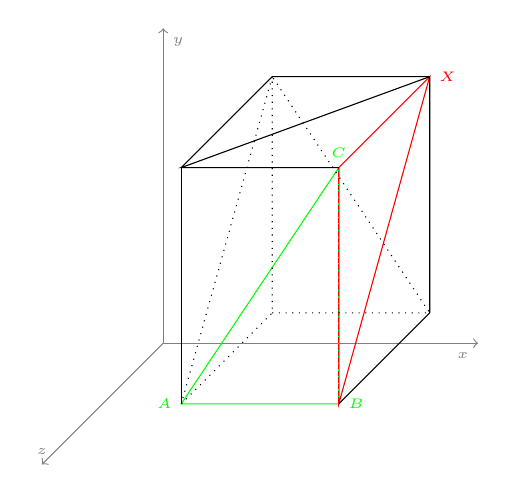
\begin{tikzpicture}

%draw the main coordinate system axes
\draw[->, gray] (0,0,0) -- (4,0,0) node[anchor=north east]{\tiny $x$};
\draw[->, gray] (0,0,0) -- (0,4,0) node[anchor=north west]{\tiny $y$};
\draw[->, gray] (0,0,0) -- (0,0,4) node[anchor=south]{\tiny $z$};


\draw[green] (1,0,2) node[anchor=east] {\tiny $A$} -- (3,0,2) -- (3,3,2) -- cycle;
\draw[red] (3,0,2) node[anchor=west, green] {\tiny $B$} -- (3,3,2) node[anchor=south, green] {\tiny $C$} -- (3,3,-1) node[anchor=west] {\tiny $X$} -- cycle;

\draw[dotted] (1,0,2) -- (1,0,-1) -- (1,3,-1) -- (1,0,2);
\draw[dotted] (1,0,-1) -- (3,0,-1) -- (1,3,-1);

\draw[green,dotted] (3,0,2) -- (3,3,2);

\draw (3,3,-1)  -- (1,3,2) -- (3,3,2);
\draw (3,3,-1) -- (3,0,-1) -- (3,0,2);

\draw (1,0,2) -- (1,3,2);

\draw (1,3,2) -- (1,3,-1) -- (3,3,-1);

\end{tikzpicture}
\end{document}